%% REPLACE sXXXXXXX with your student number
\def\studentNumber{s2447408}


%% START of YOUR ANSWERS
%% Add answers to the questions below, by replacing the text inside the brackets {} for \youranswer{ "Text to be replaced with your answer." }. 
%
% Do not delete the commands for adding figures and tables. Instead fill in the missing values with your experiment results, and replace the images with your own respective figures.
%
% You can generally delete the placeholder text, such as for example the text "Question Figure 3 - Replace the images ..." 
%
% There are 5 TEXT QUESTIONS. Replace the text inside the brackets of the command \youranswer with your answer to the question.
%
% There are also 3 "questions" to replace some placeholder FIGURES with your own, and 1 "question" asking you to fill in the missing entries in the TABLE provided. 
%
% NOTE! that questions are ordered by the order of appearance of their answers in the text, and not necessarily by the order you should tackle them. You should attempt to fill in the TABLE and FIGURES before discussing the results presented there. 
%
% NOTE! If for some reason you do not manage to produce results for some FIGURES and the TABLE, then you can get partial marks by discussing your expectations of the results in the relevant TEXT QUESTIONS. The TABLE specifically has enough information in it already for you to draw meaningful conclusions.
%
% Please refer to the coursework specification for more details.


%% - - - - - - - - - - - - TEXT QUESTIONS - - - - - - - - - - - - 

%% Question 1:
\newcommand{\questionOne} {
\youranswer{
The Vanishing Gradient Problem is present in VGG38 but not in VGG08. Figure 1 shows that both training and validation errors for VGG38 do not decrease while VGG08 shows a good decrease as the training progresses. The accuracy curve also shows a similar behaviour. Figures 2 and 3 depict the average gradients at each layer in the model. For VGG08, the gradient values are larger in the initial layers and decrease with more layers. Also, all layers have a gradient value greater than zero. But for VGG38, we see that most layers have a zero gradient except some of the final layers. This shows that when a gradient becomes zero, it is backpropagated so that all layers before it also end up with a zero gradient. From these figures we can infer that when the gradients are zero, the weights do not change and the error function does not decrease. The gradient descent never reaches a global minimum. Essentially there is no training occurring in the VGG38 model.
}
}



%% Question 2:
\newcommand{\questionTwo} {
\youranswer{
A deeper network will have a higher network capacity. It should potentially have the capability to learn more complex functions. But high network capacity can also lead to overfitting as the network becomes more tuned to the training data leading to low training errors but high testing errors. But in Figure 1 from (\cite{he2016deep}) and the results obtained above, the training error itself is very high for the deeper network. So this cannot be due to overfitting. The authors of (\cite{he2016deep}) put this issue forward as a degradation problem, where when the depth of the network increases, accuracy saturates and then degrades rapidly.
Vanishing gradients can contribute to this problem. Another factor is that deeper networks are more difficult to optimize. More layers and complex computations mean more parameters that need to be optimized. This can lead to the network getting stuck to local minima and never reaching a global minimum.}}

%% Question 3:
\newcommand{\questionThree} {
\youranswer{
Adding residual connections to a downsampling layer is not straightforward. Since the input and output have different shapes we cannot directly add them and form a residual connection. 
One way to achieve this is to apply the same downsampling operation on the identity layer(i.e., the input to block) before adding it to the output to form the residual connection. This method is easy to implement but requires more computations as we perform the downsampling twice. Also if the shapes of the output and identity do not match, we would need to use a convolution layer to correct it.
\newline
Another way would be to add a 1x1 convolution at the beginning and end of the downsampling block (before the ReLU activation). The residual connection can be added after this layer. This is called a bottleneck architecture. This ensures that the shapes of the input and output always match. Adding the 1x1 convolution reduces the number of parameters going into the convolution layers thereby reducing computation and making the model more efficient. But this method involves adding more convolutional layers to the model.}
}

%% Question 4:
\newcommand{\questionFour} {
\youranswer{
From the experiment results in Table 1, we can infer that adding Batch Normalisation or Residual connections to the VGG38 model fixed the vanishing gradient problem. The VGG38 BN model produces non-zero gradients leading to lowering errors and provides a final accuracy of about 50\% for validation data. VGG38 RC performs better than VGG38 BN with a final validation accuracy of 52\%. It should also be noted that the BN model requires more parameters to be trained than the RC model. This is because batch normalisation introduces more computations in the batch normalisation layer while residual connections do not involve any extra computation layer, it reuses the computations in the previous layers. So the RC model can complete training faster. 
The combination of both techniques is used in VGG38 BN + RC which performs better than them individually with a validation accuracy of 53\%. But the improvement is not very significant.
\newline
The gradient flow for the VGG38 BN + RC model is shown in Figure 5. We can see positive gradients on all layers. The spikes are caused by the batch normalisation layers which have a higher gradient with respect to convolution layers. But from the figure, we can conclude that the gradients are being propagated back to the initial layers uniformly in all the iterations in training.
\newline
The last two models in Table 1 use a larger learning rate of 1e-2 in training. For the VGG38 BN model, we can see that the performance has decreased i.e., the validation accuracy has come down from 50\% to 47\%. The degradation is more evident in the training data where the accuracy has come down from 59\% to 52\%. For the VGG38 BN + RC model with learning rate 1e-2, we see the best validation accuracy rate of 56\%. There is also a significant improvement from the VGG38 BN model with the same learning rate. But interestingly, looking at the training curves for the VGG38 BN + RC model in Figure 4, we can see that the validation loss and accuracy fluctuate and do not remain steady, unlike the training loss and accuracy. It does achieve a better validation accuracy of 60\% in the second last epoch. This could be because of the high value of the learning rate, which causes the model to bounce around the optimal solution and not converge stably. In the VGG38 BN +RC model with a learning rate of 1e-3, we can see that it has not reached the optimal solution yet, which means that the learning rate is too small. 
\newline
Comparing the different models it seems that the VGG38 BN + RC gives a better performance. However, the learning rates used are not optimal. Further experiments can be performed with different learning rates. Since 1e-3 was too small and 1e-2 was too large, we can run the model with learning rates 5e-3, 2.5e-3 and 7.5e-3 to find the optimal value.
Another experiment can be done to run a VGG38 RC model with learning rate 1e-2 to check if the behaviour observed with learning rate 1e-3 can be replicated where RC performs better than BN. This experiment can also validate whether the combination of BN + RC is better than only RC. If the improvement is not very significant, it can indicate residual connections alone can be used without the additional overhead of using batch normalisation. 

}
}


%% Question 5:
\newcommand{\questionFive} {
\youranswer{
The objective of this report was to understand the vanishing gradient problem observed in deep neural networks and identify techniques to mitigate it. We analysed the VGG08 and VGG38 models and discovered that the vanishing gradient problem occurs only in the VGG38 model. Two techniques were identified to solve this problem, Batch Normalisation and Residual Connections. We applied both these approaches in the VGG38 model and gathered the results.
\newline
The results confirmed that both batch normalisation and residual connections can help mitigate the vanishing gradient problem. The model with only residual connections performed better than the one with only batch normalisation. Batch normalisation requires more parameters in the model leading to more computations and training time.
But using a combination of both techniques gives the best-performing model. We ran the models with two different learning rates, 1e-2 and 1e-3. We found that 1e-2 was too large leading to the model not converging. We also found that 1e-3 was too small since the model did not reach the optimal solution in 100 epochs.  
\newline
The VGG38 model can be run with different learning rates to improve its performance. In the above experiments, we have not added residual connections to the downsampling layers. Adding this can improve the model. From Figure 1, it is also clear that there is a divergence between the training and validation accuracies/losses. This could be due to overfitting. A regularisation technique like dropout can be used to reduce the generalisation gap.
}
}


%% - - - - - - - - - - - - FIGURES - - - - - - - - - - - - 

%% Question Figure 3:
\newcommand{\questionFigureThree} {
%
\begin{figure}[t]
    \centering
    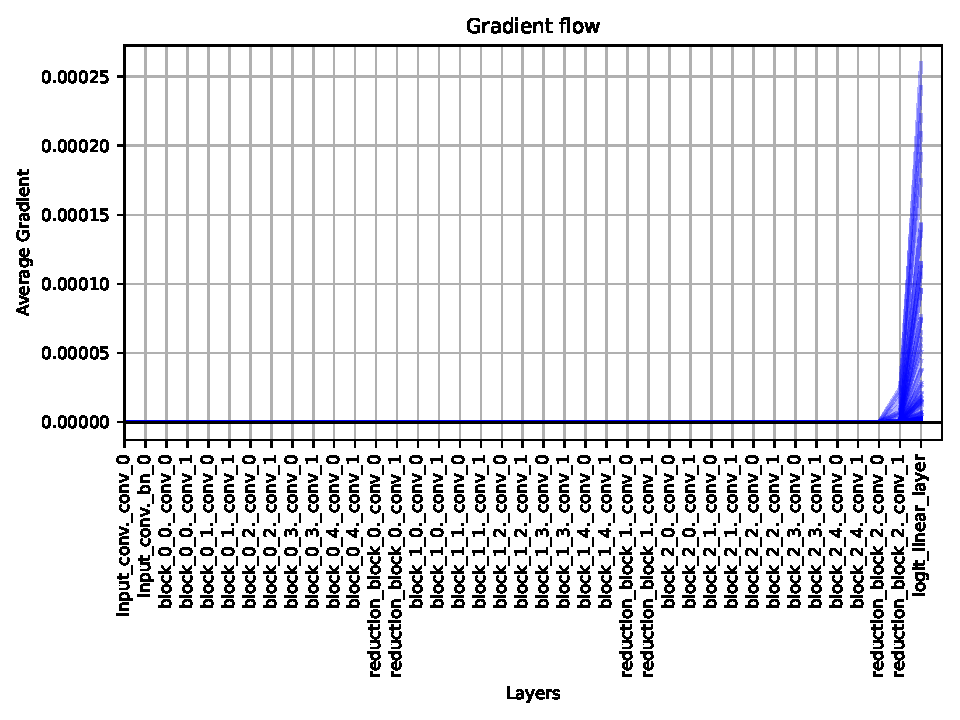
\includegraphics[width=\linewidth]{figures/grad_flow_vgg38.pdf}
    \caption{Gradient Flow on VGG38}
    \label{fig:grad_flow_38}
\end{figure}
}

%% Question Figure 4:
\newcommand{\questionFigureFour} {
%
\begin{figure}[t]
    \centering
        \begin{subfigure}{\linewidth}
        \centering
        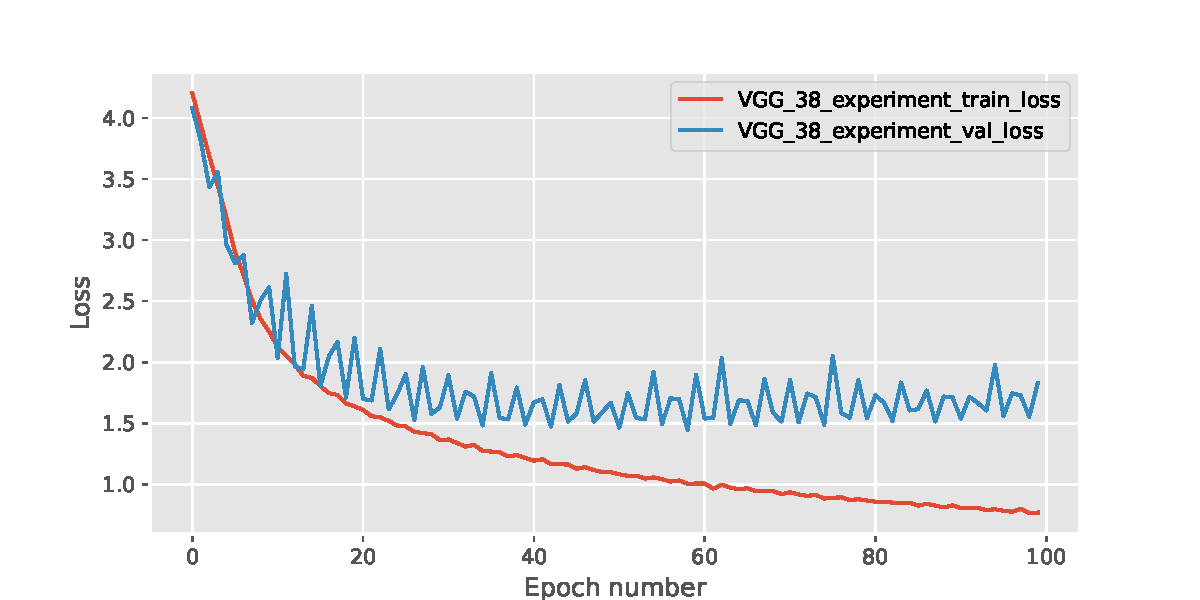
\includegraphics[width=\linewidth]{figures/VGG_38_BN_RC_loss_performance.pdf}
        \caption{Cross entropy error per epoch}
        \label{fig:loss_curves}
    \end{subfigure}

    \begin{subfigure}{\linewidth}
        \centering
        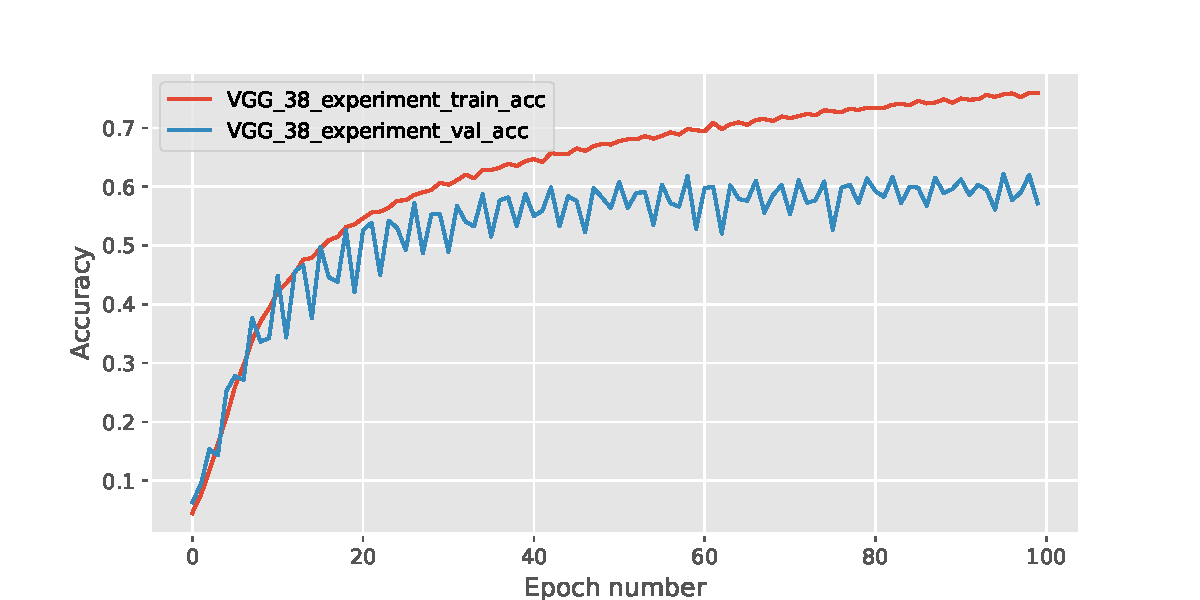
\includegraphics[width=\linewidth]{figures/VGG_38_BN_RC_accuracy_performance.pdf}
        \caption{Classification accuracy per epoch}
        \label{fig:acc_curves}
    \end{subfigure}
    \caption{Training curves for VGG38 with Batch Normalisation (BN) and Residual Connections (RC) in terms of (a) cross-entropy error and (b) classification accuracy}
    \label{fig:grad_flow_bestModel}
\end{figure}

}

%% Question Figure 5:
\newcommand{\questionFigureFive} {
%
\begin{figure}[t]
    \centering
    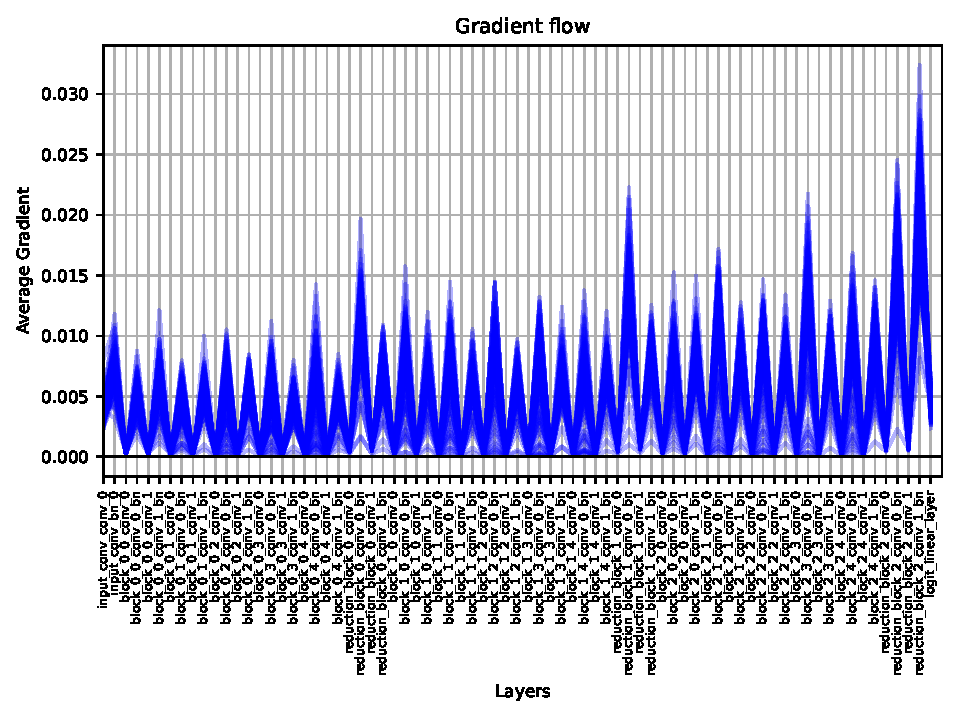
\includegraphics[width=\linewidth]{figures/grad_flow_vgg38_BN_RC.pdf}
    \caption{Gradient Flow on VGG38 with Batch Normalisation (BN) and Residual Connections (RC)}
    \label{fig:grad_flow_bestModel}
\end{figure}

}

%% - - - - - - - - - - - - TABLES - - - - - - - - - - - - 

%% Question Table 1:
\newcommand{\questionTableOne} {
%
\begin{table*}[t]
    \centering
    \begin{tabular}{lr|ccccc}
    \toprule
        Model                   & LR   & \# Params & Train loss & Train acc & Val loss & Val acc \\
    \midrule
        VGG08                   & 1e-3 & 60 K      &  1.74      & 51.59     & 1.95     & 46.84 \\
        VGG38                   & 1e-3 & 336 K     &  4.61      & 00.01     & 4.61     & 00.01 \\
        VGG38 BN                & 1e-3 & 339 K     &  1.40     & 59.16      & 1.98      & 49.88 \\
        VGG38 RC                & 1e-3 & 336 K     &  1.33      & 61.52     & 1.84     & 52.32 \\
        VGG38 BN + RC           & 1e-3 & 339 K     &  1.26      & 62.99     & 1.73     & 53.76 \\
        VGG38 BN                & 1e-2 & 339 K     &  1.70      & 52.28     & 1.99     & 46.72 \\
        VGG38 BN + RC           & 1e-2 & 339 K     &  0.80      & 75.22     & 1.86     & 56.84 \\
    \bottomrule
    \end{tabular}
    \caption{Experiment results (number of model parameters, Training and Validation loss and accuracy) for different combinations of VGG08, VGG38, Batch Normalisation (BN), and Residual Connections (RC), LR is learning rate.}
    \label{tab:CIFAR_results}
\end{table*} 

}

%% END of YOUR ANSWERS
